\chapter{Guida all'uso}
  \begin{abstract}
    Come detto \hi{InfoPoint} è suddiviso nelle 2 componenti di \hi{server} e \hi{client}. Di seguito riportiamo, per entrambi, l'analisi e le scelte effettuate durante il loro sviluppo
  \end{abstract}

  \section{Guida al Server}
    \subsection{Funzionalità}
      Il Sistema, deve offrire, una serie di funzionalità:
      \begin{itemize}
        \item Possibilità di connessione concorrente;
        \item Possibilità di potersi registrare alla piattaforma\footnotemark \footnotetext{Le credenziali vengono salvate facendo uso di un Database, che risulta molto più affidabile di un semplice file di testo};
        \item Possibilità di usufruire dei contenuti in base alla tipologia di utente, in modo da permette un focus diverso in base alle sue caratteristiche\footnotemark \footnotetext{Ricordiamo che il bacino degli utenti che possono fare uso del sistema può variare da scolaresche, famiglie o esperti} ;
      \end{itemize}

    \subsection{Scelte implementative}
        Seguendo il concetto del \emph{DIVIDE ET IMPERA}\footnotemark \footnotetext{Metodologia per la risoluzione di problemi $\rightarrow$ Il problema viene diviso in sottoproblemi più semplici e si continua fino a ottenere problemi facilmente risolvibili. Combinando le soluzioni ottenute si risolve il problema originario.} si è scelto di spezzare le varie funzionalità che vengono messe a disposizione per rendere il codice facilmente manutenibile ed evitare lo stato di codice monolitico\footnotemark \footnotetext{Che risulta notoriamente più difficile da gestire e modificare nel tempo}.

        In particolare l'implementazione fa ampiamente uso di codice sviluppato in \hi{C POSIX}, che permette l'utilizzo di funzionalità
        e \hi{system call}\footnotemark su cui si basa l'intera code-base: send, recv, socket, thread pool, mutex, argp \dots

        \footnotetext{Una chiamata si definisce, appunto, \hi{di sistema}, quando fa uso di servizi e funzionalità a livello kernel del sistema operativo in uso.}
    \subsection{Tecnologie e strumenti utilizzati}
      Per una migliore gestione del Sistema, si è fatto uso di una serie di strumenti.

      Durante lo sviluppo si è fatto uso dell'utility \hi{cmake}\footnotemark \footnotetext{Per maggiori informazioni visitare il seguente \href{https://cmake.org/}{sito}} , tool modulare che permette la generazione di un \hi{Makefile}\footnotemark

      automatizzato.

      \footnotetext{Che contiene tutte le direttive utilizzate dall'utility make, che ne permettono la corretta compilazione}

      Per la fase di deploy invece si è fatto uso di \hi{docker}, tool che permette l'esecuzione di programmi in maniera containerizzata.

      Come sperato, avendo adottato entrambe le strategie non si sono riscontrati problemi durante il passaggio da un ambiente locale (di testing) a uno decentralizzato (production ready).
    \subsection{Memorizzazione dei dati}
    Per essere sempre in linea con le nuove tendenze e tecnologie si è scelto di abbandonare il classico approccio basato su un collegamento ad una base di dati relazionale, preferendo un approccio di tipo \hi{NOSQL}\footnotemark , \footnotetext{Che a differenza dei classici DBMS relazioni (che offrono un approccio \texttt{relazione} ai dati) offre un approccio al documento, rendendo il design più semplice} che offre una maggiore elasticità \footnotemark \footnotetext{Per loro natura infatti sono pensati per lavorare in situazioni di alto carico di lavoro pur mantenendo basse latenze}
    e scalabilità\footnotemark nel tempo.

    \footnotetext{Per la loro natura offrono una forte resilienza a situazioni di fault, considerando il focus scelto (AP) nel \href{https://www.ibm.com/it-it/cloud/learn/cap-theorem}{\hi{CAP}} (Consistency-Availability-Partition Tolerance) }
    \newpage
  \section{Guida al Client}
    Prestando particolare attenzione alla semplicità di utilizzo che un'applicazione mobile deve garantire si è scelto di fare uso di un’interfaccia snella e lineare.
    \subsection{Primo avvio}
      All'avvio all'utente è richiesto di registrarsi o accedere alla piattaforma, facendo uso della classica combinazione mediante \hi{username} e \hi{password}.

    \subsection{Post registrazione}
      In seguito ad una corretta registrazione/accesso all'utente viene mostrata la \hi{HomePage}, nella quale ha la possibilità di visualizzare:
      \begin{itemize}
        \item L'elenco delle \hi{artwork} presenti nel museo;
        \item La possibilità di poter ricercare le opere in base a
          \begin{itemize}
            \item Nome;
            \item Autore;
            \item Data;
          \end{itemize}
        \item Il proprio profilo;
        \item L'accesso diretto alle artwork preferite.
      \end{itemize}
    \subsection{Memorizzazione delle informazioni}
    In linea con il design pattern \hi{MVVM} \footnotemark \footnotetext{(Model–view–viewmodel), pattern nel quale viene astratto lo stato di view (visualizzazione) e comportamento}, si è fatto uso delle \href{https://developer.android.com/reference/android/content/SharedPreferences}{\hi{SharedPreferences}} per il salvataggio e la gestione di componenti chiave quali:
      \begin{itemize}
        \item Credenziali dell'utente;
        \item Variabili d'ambiente;
        \item Variabili di stato;
      \end{itemize}
    
    \newpage
    \subsection{Modelli di dominio}
      \begin{center}
        \hi{Class Diagram}

            Di seguito riportiamo il diagramma delle classi di Analisi prodotto durante lo sviluppo della piattaforma InfoPoint

            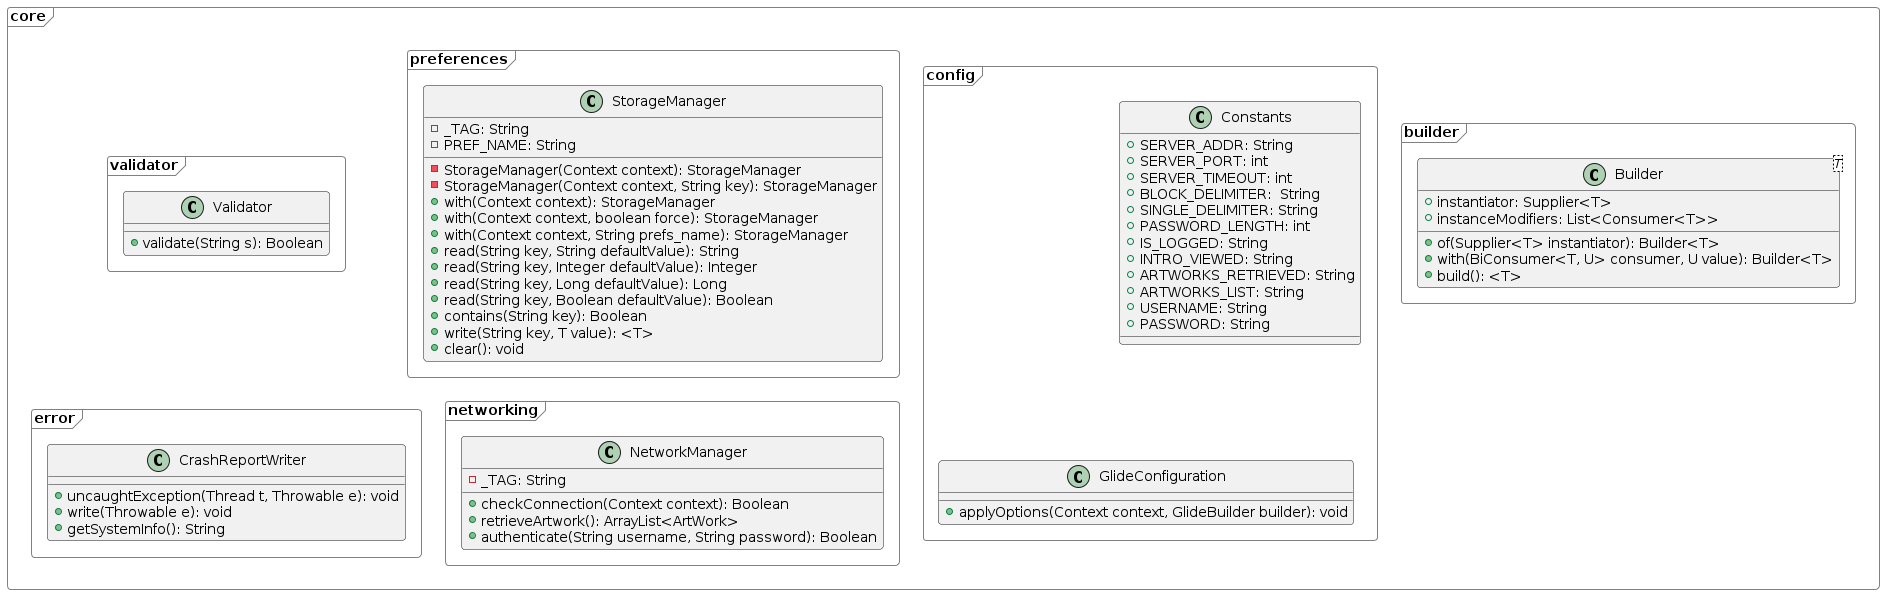
\includegraphics[width=19cm, height=19cm, keepaspectratio]{content/img/core.png}

            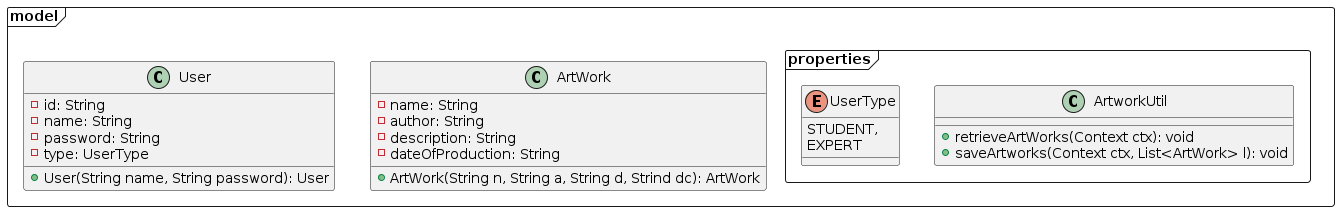
\includegraphics[width=19cm, height=19cm, keepaspectratio]{content/img/models.png}

            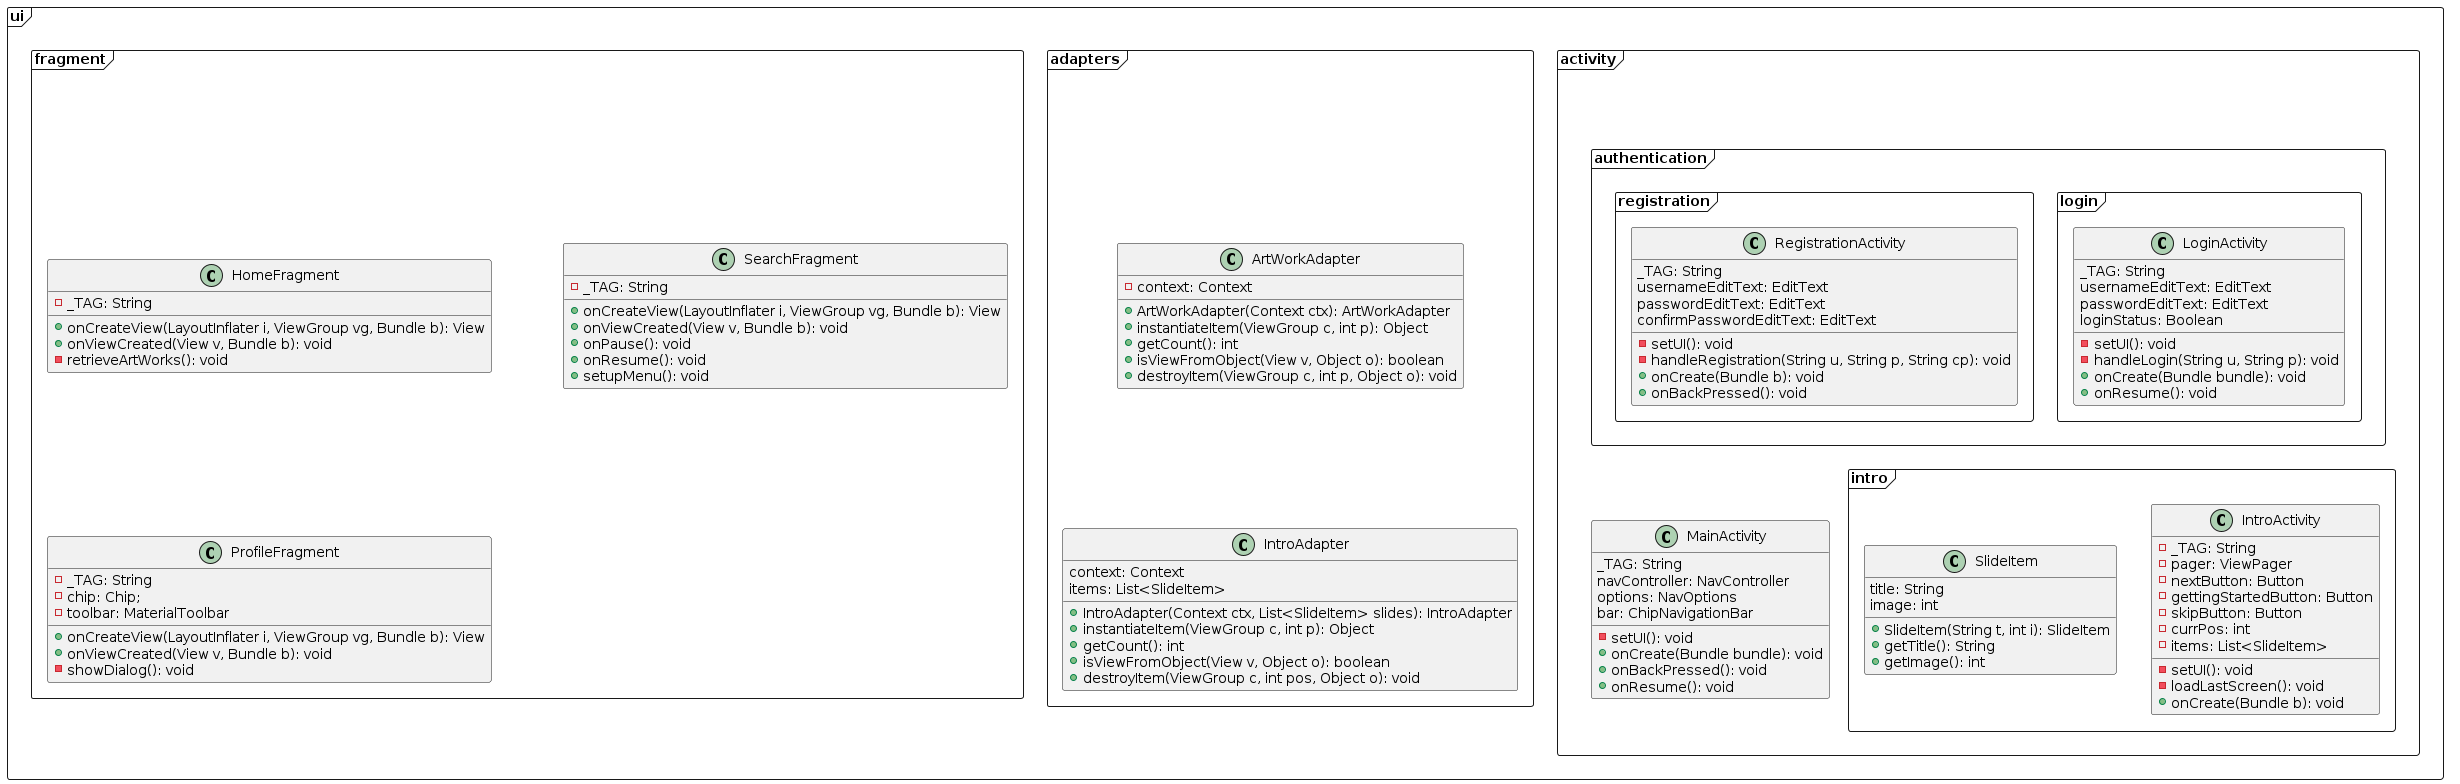
\includegraphics[width=19cm, height=19cm, keepaspectratio]{content/img/ui.png}
      \end{center}
